\section{Auswertung}
\label{sec:aus}

\subsection{Dampfdruckkurve Tiefdruck}
Zunächst wird die Dampfdruckkurve für Drücke im Bereich von 30 $\si{\milli\bar}$ bis circa 1000 $\si{\milli\bar}$ untersucht. Das Vorgehen wird in \autoref{sec:dis} beschrieben.
Die aufgenommenen Messwerte sind in der \autoref{tab:1} aufgelistet.

\begin{table}
    \centering
    \caption{Messwerte vom Druck $p$, sowie der Wassertemperatur $T_W$ und der Lufttemperatur $T_L$ }
    \label{tab:1}
    \begin{tabular} {S[table-format=2.0] S[table-format=3.1] S[table-format=3.0]}
        \toprule
        {$p \mathbin{/} \si{\milli\bar}$}&{$T_W \mathbin{/} \si{\celsius}$} & {$T_L \mathbin{/} \si{\celsius}$} \\
    \midrule
    74  & 30   &   25   \\
    86  & 35   &   36   \\
    96  & 40   &   38   \\
    110 & 45   &   40   \\
    127 & 50   &   49   \\
    160 & 55   &   54   \\
    200 & 60   &   59.5 \\
    247 & 65   &   64   \\
    307 & 70   &   70   \\
    372 & 75   &   71   \\
    460 & 80   &   82   \\
    550 & 85   &   99   \\
    648 & 90   &   106.5\\
    \bottomrule
\end{tabular}
\end{table}

\noindent
Die gemessenen Werte werden in ein Diagramm (\ref{fig:1}) eingetragen und mithilfe einer Augleichsgeraden der Form
\begin{equation}
    y = m*x + n 
\end{equation}

\noindent
gefittet, wobei sich mit der \autoref{eqn:claui} %Logerithmus
für $m=-\frac{L}{R}$ und für $y=\frac{p}{p_0}$ ergibt. 

\begin{figure}
    \centering
    \caption{Messdaten und Fit für die Temperatur gegen den Druck}
    \label{fig:1}
    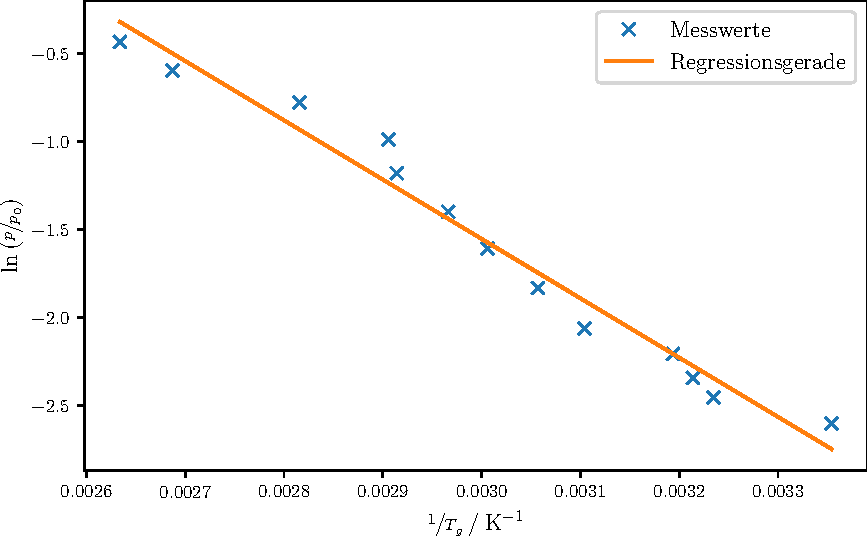
\includegraphics{Daten/tiefdruck.pdf}
\end{figure}

\noindent
Mithilfe der Ausgleichsgerade ergibt sich für 
\begin{align*}
    m &= \SI{-3369.90(17463)}{\kelvin}\\
    b &= \SI{0.65(53)} \, .
\end{align*}

\noindent 
Daraus lässt sich die Verdampfungswärme $L$ mithilfe der Gaskonstante $R = \SI{8,314462618}{\joule\per\mole\per\kelvin}$\cite{gasconstant} errechnen zu 
\begin{equation*}
    L = \SI{2.80189(15)e04}{\joule\per\mole} \, .
\end{equation*}

\subsection{äußere Verdampfungswärme}
Mithilfe der Allgemeinen Gasgleichung 
\begin{equation*}
    V_D(p,T) =R \frac{T}{p} 
\end{equation*}

\noindent
lässt sich die Verdampfungswärme $L_\text{a} = RT$ bei $T = \SI{373}{\kelvin}$ abschätzen. Die Arbeit , welche notwendig ist molekularen Anziehungskräfte bei der Verdampfung zu Überwinden, heißt 
$L_\text{i}$ und ist gegeben durch $ L_\text{i} = L - L_\text{a}$. Daraus folgt, dass der Zusammenhang
\begin{align*}
    \frac{L_\text{i}}{N_\text{A}} =& \frac{L - L_\text{a}}{N_\text{A}} = \frac{L - RT}{N_\text{A}} \\
    =& \frac{\SI{2.80(15)e04}{\joule\per\mole} - \SI{8,314462618}{\joule\per\mole\per\kelvin} \cdot \SI{373}{\kelvin}}{\SI{6.02214076e23}{\per\mole}} \\
    =& \SI{0.258(15)}{\electronvolt} \, ,
\end{align*}

\noindent
gilt, wobei $N_\text{A}$ die Avogadro-Konstante ist.

\subsection{Hochdruck}
Für die Auswertung der Abhängigkeit der Verdampfungswärme von der Temperatur bei Drücken von $p \, > \, 1\si{\bar}$ werden wieder Messwerte aufgenommen, jedoch in einem anderen Versuchsaufbau. Dieser wird ebenfalls
in \autoref{sec:dis} erläutert. Die Messwerte sind in der \autoref{tab:2} aufgelistet.

\begin{table}
    \centering
    \caption{Messwerte vom Druck $p$ bei der Temperatur $T$}
    \label{tab:hochdruck}
    \begin{tabular} {S[table-format=2.0] S[table-format=3.0]}
        \toprule
        {$T \mathbin{/} \si{\celsius}$} & {$p \mathbin{/} \si{\bar}$}\\
    \midrule
    120 & 1  \\
    132 & 2  \\
    141 & 3  \\
    150 & 4  \\
    156 & 5  \\
    161 & 6  \\
    167 & 7  \\
    172 & 8  \\
    177 & 9  \\
    180 & 10 \\
    184 & 11 \\
    187 & 12 \\
    191 & 13 \\
    192 & 14 \\
    195 & 15 \\
    \bottomrule
\end{tabular}
\end{table}

\noindent
Zunächst werden die Messwerte wieder, wie im Kapitel davor, in eine \autoref{fig:2} eingetragen und mit einer Funktion gefittet. Diese ist jedoch vom Grad 3, sodass der Ansatz wie folgt
aussieht
\begin{equation*}
    y = kx^3+bx^2+cx+d \, ,   
\end{equation*}

\noindent
wobei $y = p(T)$ und $ x=T$ entspricht. Der Fit ergibt für die Werte %
\begin{align*}
    k &= \SI{1.93(50)}{\pascal\per\kelvin\tothe{3}}         \, ,        \\
    b &= \SI{-2299.79(64999)}{\pascal\per\kelvin\tothe{2}}  \, ,        \\ 
    c &= \SI{923918.92(28013445)}{\pascal\per\kelvin}       \, ,         \\
   \text{und } d &= \SI{-124836792.62(4018067192)}{\pascal\per\kelvin} \, .
\end{align*}

\begin{figure}
    \centering
    \caption{Messdaten und Fit für die Temperatur gegen den Druck}
    \label{fig:2}
    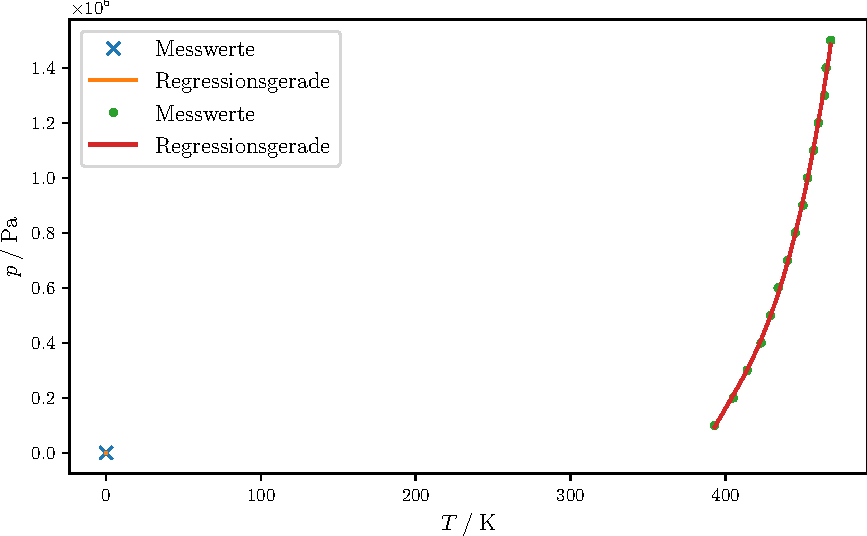
\includegraphics{Daten/hochdruck.pdf}
\end{figure}

\noindent
Um die Abhängigkeit der Verdampfungswärme von der Temperatur berechnen zu können wird die Clausius-Clapeyronsche Gleichung (\ref{eqn:clau}) nach
\begin{equation}
    T \, (V_D - V_F) \, \frac{\text{d}p}{\text{d}T} = L 
\end{equation}

\noindent
umgestellt und mit der Näherung 
\begin{equation*}
    \left( p + \frac{a}{V^2}\right) V = RT
\end{equation*}

\noindent
für $V_\text{D}$ kann die Verdampfungswärme bestimmt werden zu ($V_F$ ist vernachlässigbar)
\begin{equation}
    L = \left( \frac{RT}{2p} \pm \sqrt{\frac{R^2T^2}{4p^2} - \frac{a}{p}}\right)\left( 3kT^2 + 2bT + c \right) \, ,
\end{equation} 

\noindent
mit $a = \SI{0.9}{\joule\metre\tothe{3}\per\mole\squared}$. Mithilfe der 2 Formeln dür $L$ lässt sich der Zusammenhang der zwischen Temperatur und Verdampfungswärme graphisch 
in \autoref{fig:3} dargestellen.

\begin{figure}
    \centering
    \caption{errechnetes $L_+$ und $L_-$ gegen die Temperatur}
    \label{fig:3}
    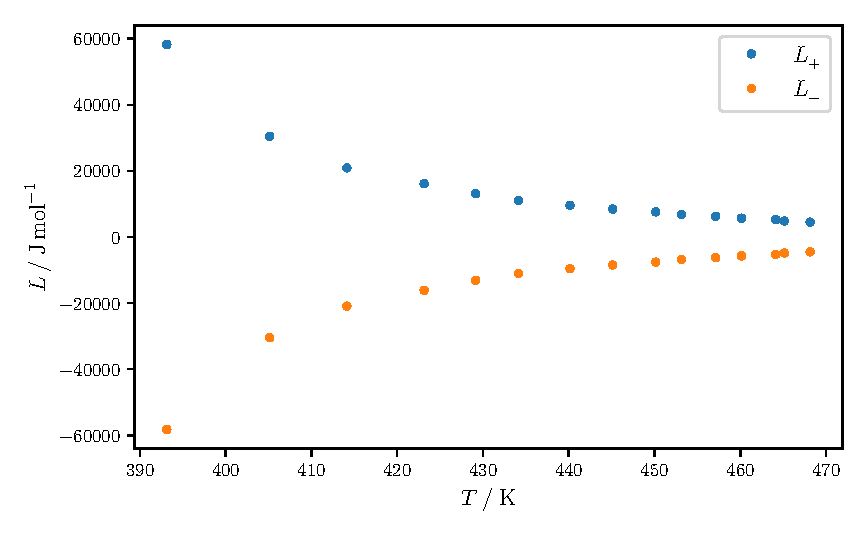
\includegraphics{Daten/zeitabhaengigkeit.pdf}
\end{figure}

